\documentclass{beamer}

% for themes, etc.
\mode<presentation>
{ \usetheme{metropolis} }
%{ \usetheme{boxes} }

\usepackage{times}  % fonts are up to you
\usepackage{graphicx}

% these will be used later in the title page
\title{South Africa ALICE Computing and WLCG and grid}
\author{Sean Murray \\
    ALICE \\
    CHPC,CSIR \\
    University of Cape Town 
}
\date{May 4 2017}

% note: do NOT include a \maketitle line; also note that this title
% material goes BEFORE the \begin{document}

% have this if you'd like a recurring outline
\AtBeginSection[]  % "Beamer, do the following at the start of every section"
{
\begin{frame}<beamer> 
\frametitle{Outline} % make a frame titled "Outline"
\tableofcontents[currentsection]  % show TOC and highlight current section
\end{frame}
}

\begin{document}

% this prints title, author etc. info from above
\begin{frame}
\titlepage
but first the important stuff.
\end{frame}

\begin{frame}
    \frametitle{Happy Starwars Day.}
    \centering{
    \includegraphics[scale=0.25]{StarWars.jpg}\\
    \includegraphics[scale=0.1]{starwars1.jpg}
}
\end{frame}
\section{Current Status (last year)}
\begin{frame}
    \frametitle{Location}
    \centering{
    \includegraphics[scale=0.35]{ALICEGridSites.png}
}
\end{frame}
\begin{frame}
\frametitle{Commitments}
According to Tender :
\begin{itemize}
  \item ALICE 600 cores
  \item ATLAS 600 cores
  \item ALICE 400TB [383TB]
  \item ATLAS 400TB [248TB]
\end{itemize}
According to :
https://wlcg-rebus.cern.ch/apps/pledges/resources/
\begin{itemize}
  \item 6000 HEPSPEC06 cores (560 of our cores)
  \item 100TB storage
  \item All ALICE.
\end{itemize}
\end{frame}

\begin{frame}
  \frametitle{Computing Infrastructure}
  \centering{
  \includegraphics[scale=0.30]{CHPCConnectivityDiagram.jpg}
  }
\end{frame}
\begin{frame}
  \frametitle{Current hardware}
  \begin{itemize}
    \item 50 nodes of 48 cores 192GB RAM and 1.6TB of SSD, 2x bonded 1G ethernet
    \item 34 nodes of 48 cores 96GB RAM and 1TB, QDR infiniband, 6 lost to another project
    \item 100TB of Lustre on the 34 nodes with QDR infiniband. now dead.
    \item 9 management servers, lower spec 
  \begin{itemize}
    \item compute element (head node,ce),
    \item storage element 2 redirectors, 2 storage nodes with direct attached multipath storage
    \item authentication, user interface (gone), monitoring, provisioning. 
  \end{itemize}
  \end{itemize}
\end{frame}

\begin{frame}
  \frametitle{Current Storage}
  \begin{itemize}
    \item 383TB EOS for ALICE, down from 440TB
    \item 252 TB EOS for ATLAS, down from 400TB
    \item 107 TB lustre for 34 nodes. dead
    \item 104 TB EMC for ATLAS. dead and now revived.
  \end{itemize}
Reduction in data sizes is due to reorganisation for reliability.
\end{frame}

\begin{frame}
  \frametitle{Improvements}
  Since my epoch \ldots
  \begin{itemize}
    \item Fixed ALICE error rates, mostly, or know the cause with solutions pending.
    \item ALICE concurrent jobs from 700 to 2100 (briefly).
    \item max out bandwidth now regularly in both directions, and now storage is getting hit.
    \item ATLAS running pilot jobs. 
    \item Storage cleaned up.
    \item New storage quoting, now changed to intergrated RFP.
    \item Plan in place to reinstall entire site, and being tested.
        \item xcat replaced by foreman.
  \end{itemize}

\end{frame}

\begin{frame}
  \frametitle{Transparency}
  Historically this has not been great, so \ldots
  \begin{itemize}
    \item Federated logins to zabbix and grafana, and public.
    \item All code on github in line with AAROC, after getting burnt at last employer.
    \item All issues PUBLIC on github, redmine is more admin than I want.
    \item A few privacy problems need to be ironed out still, like network diagrams, and passwords.
    \item AAROC slack channels for reporting everything.
  \end{itemize}
\end{frame}


\begin{frame}
  \frametitle{Current Performance last year}
    \includegraphics[scale=0.15]{ALICERunning1Year.png}
\begin{itemize}
  \item 890k ALICE jobs in last year, 465 the previous year.
  \item 980 Avg concurrent jobs up from 704.
  \item 91TB of 383TB 
  \item 235.1TB(139) in 404.5TB(97) out.
  \item Average 8.9MB/s in and 14.3MB/s
\end{itemize}
\includegraphics[scale=0.25]{NGIAccounting-ShowingAugustPeak.jpg}
\end{frame}

\begin{frame}
    \frametitle{Graph of Storage Use}
    \includegraphics[scale=0.25]{CHPCEOSUsage.png}
\end{frame}

\begin{frame}
  \frametitle{Availability / Reliability}
\vspace{0.5cm}
\centering{
\begin{tabular}{|c|r|}
  Function     &  Last 365 days \\ \hline 
  Availability &  98  \\ \hline
  Reliability  &  99  \\ \hline
  Storage & 94.5 \\ \hline
\end{tabular}
}\\
\vspace{0.5cm}
Storage down time is primarily due to storage test failures due to network starvation.
\end{frame}

\begin{frame}
    \begin{itemize}
            \item bouncy running jobs is due to chasing the queue down and up.
    \item error\_e caused by errors of things taking too long to get data.
    \item random increases in jobs due to no jobs matching (graphs) and 
    \item can not start more then about 50 jobs at a time, to stay stable.
        \item This is all due to network problems, a standing joke, the network is for all on site.
    \end{itemize}
\end{frame}

\begin{frame}
\frametitle{Downtimes}
The big ones are, ignoring network starvation :
\begin{itemize}
  \item [21 May] Site Power upgrade whole weekend.
  \item [22 Jun] General Power failure, storage out for 2 days, SAM tests in unknown for 1 week.
  \item [10 Oct] power test down for 1 day.
\end{itemize}
\end{frame}

\begin{frame}
  \frametitle{Data Traffic Mid June}
  \centering{
  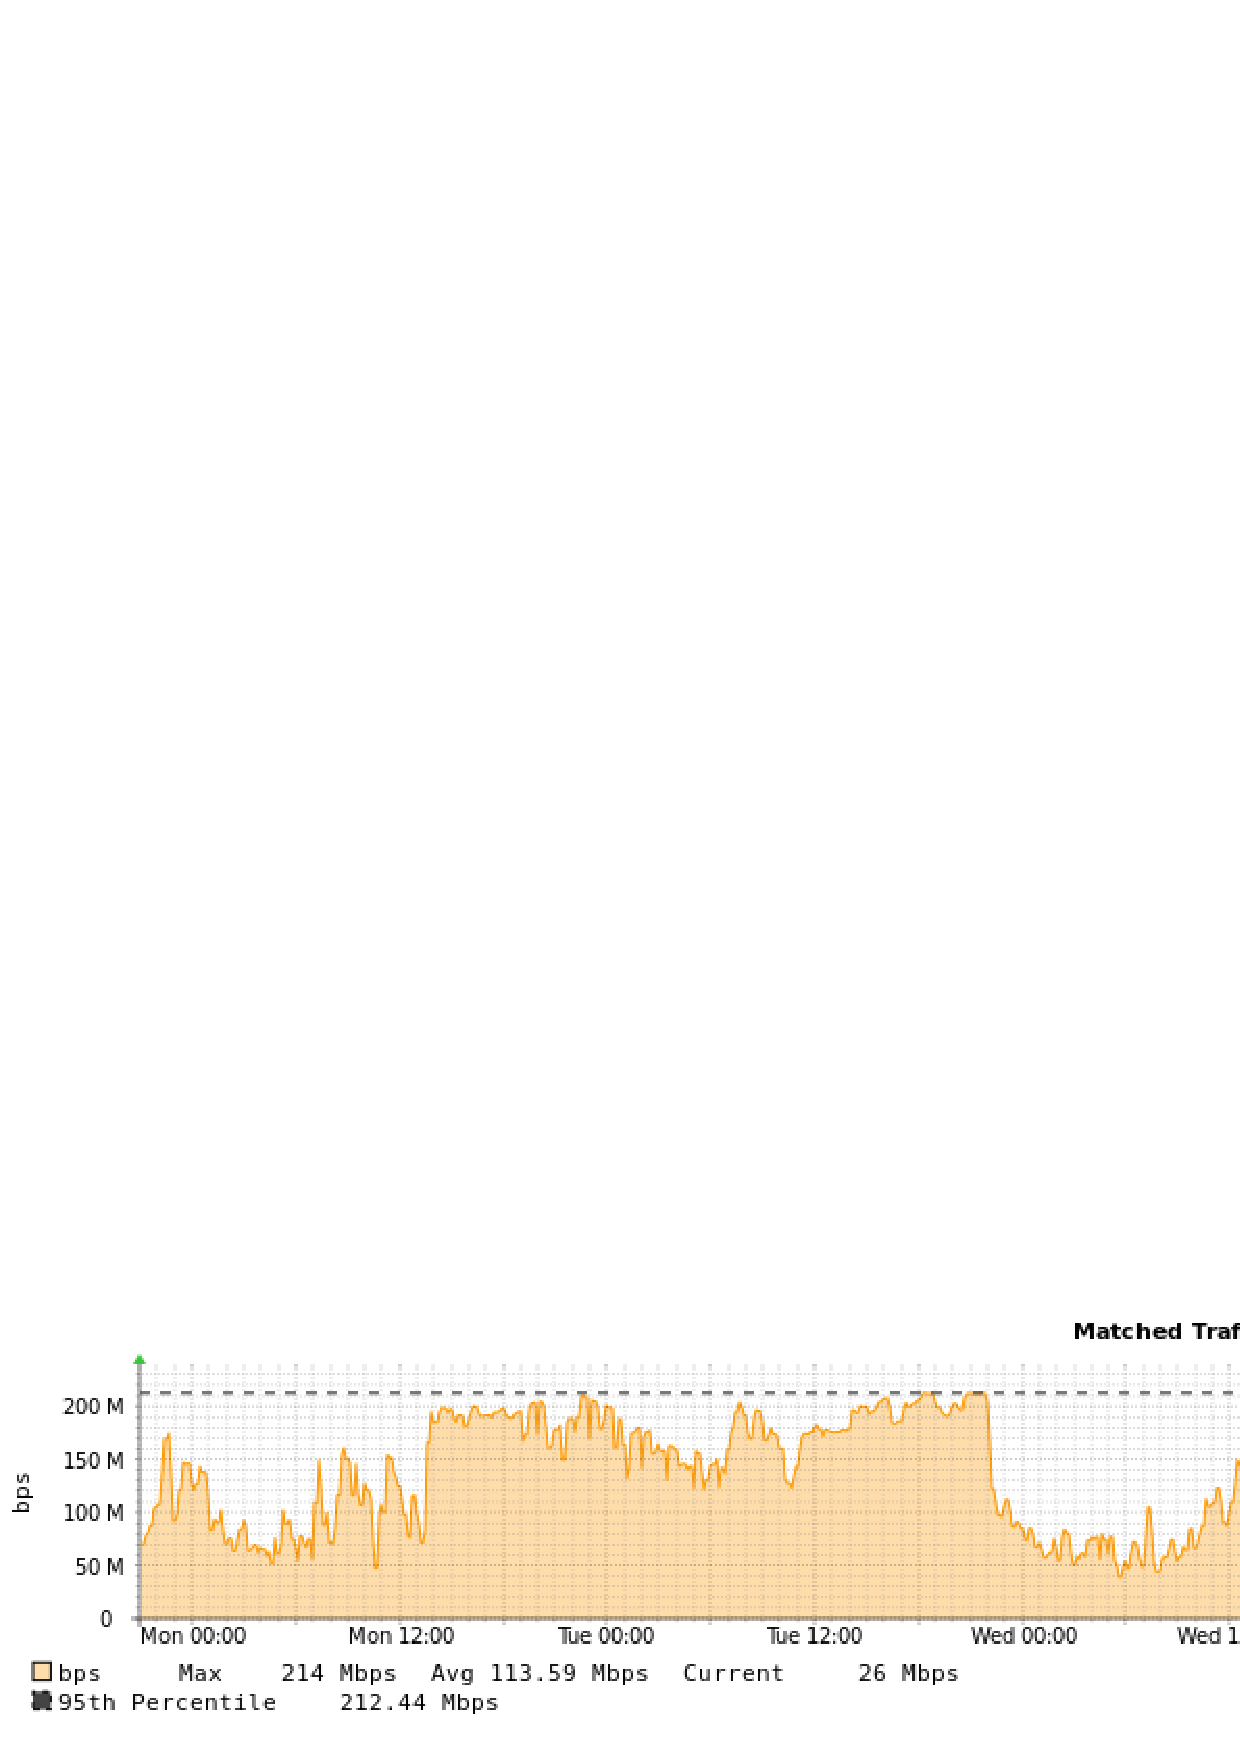
\includegraphics[scale=0.25]{wacsinmidjun.pdf}\\
  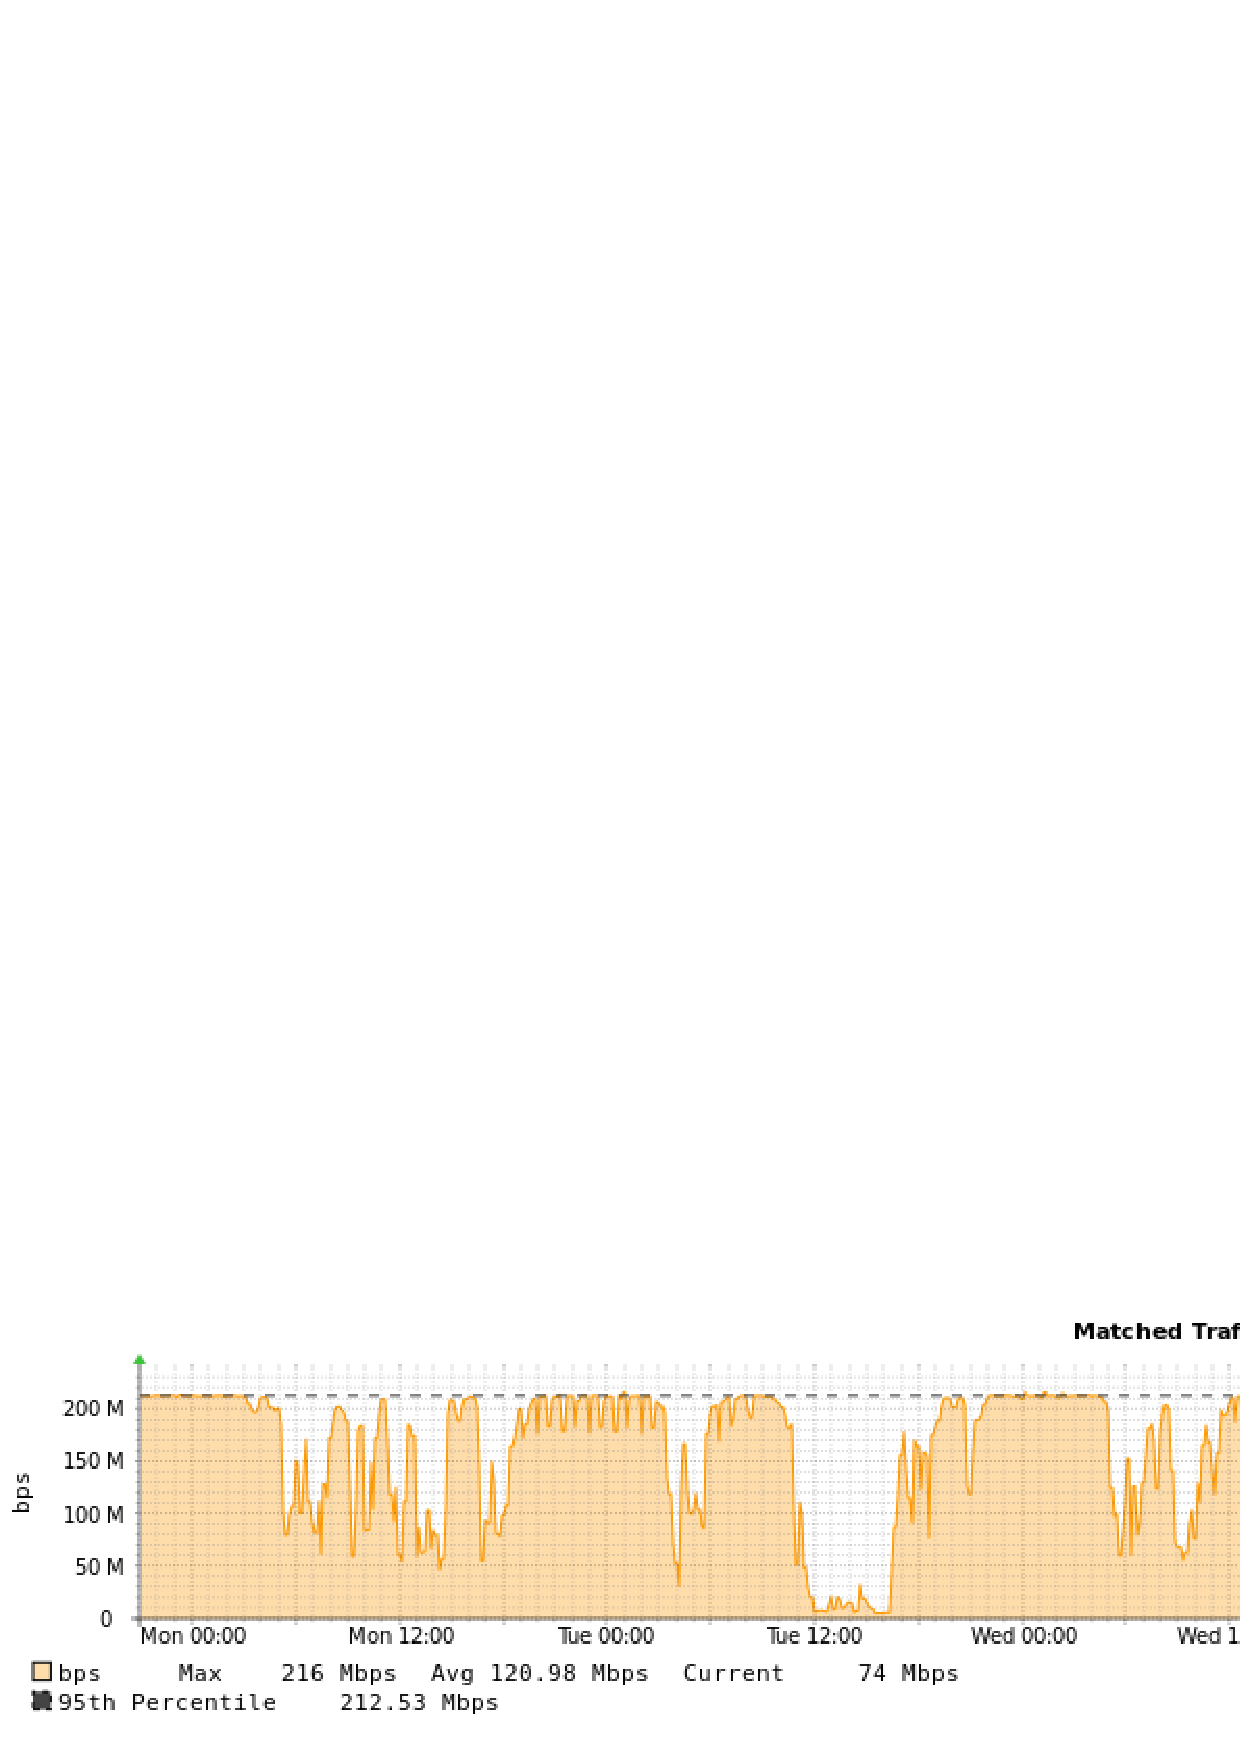
\includegraphics[scale=0.25]{seacomoutmidjun.pdf}
  }
\end{frame}
\begin{frame}
    \frametitle{TENET permiter graphing}
  \centering{
  \includegraphics[scale=0.25]{LastMonthTenetIn.png}\\
  \includegraphics[scale=0.25]{LastMonthTenetOut.png}
  }
\end{frame}

\begin{frame}
    \frametitle{Network maximisation}
It was always a concern for when our storage becomes sufficiently full to be usefull to others.
    \begin{itemize}
            \item March 2, problems in Mexico and our storage got hit outgoing, 2 days cpu down
            \item March 4 another person liked our data, 2 days cpu down.
                \item Then, because our storage is under utilised, it became a replication site.
                    \item When in an out on storage is maxed out the compute blows up....
    \end{itemize}
    \includegraphics[scale=0.15]{ALICEMonaLisa-ShowingStartingJobs.png}
\end{frame}
\begin{frame}
    \frametitle{Status this morning}
    \includegraphics[scale=0.25]{ALICEGrafanaStatus-20170503.png}\\
\end{frame}
\begin{frame}
    \frametitle{Another example }
    \includegraphics[scale=0.25]{ALICETier2-Status-AttemptToStart50JobsAndBlowsUpUnknownReason-FailedFeedbackLoop.png}
\end{frame}
\begin{frame}
    \frametitle{Storage Swamping network}
    Network was bad and then since March the storage has made things worse.\\
    \includegraphics[scale=0.25]{StorageNetworkUsage.png}
\end{frame}
\begin{frame}
    \frametitle{Processing Today}
    \includegraphics[scale=0.25]{ALICEStatus-20170504.png}
\end{frame}

\begin{frame}
    \frametitle{provided and (required)}
\vspace{0.5cm}
\centering{
\begin{tabular}{|c|c|c|c|c|}
    Resource          &  2016          & 2017              & 2018         & 2019 \\ \hline 
    CPU     kHS06     &  7.5 (6)       & 7.5 (7.5)         & 7.5(8.09)    & 7.5(12.35)  \\ \hline
    Storage    TB     &  384 (550)     &  384 (682)  & 384(990)   & 384(1100)  \\ \hline
\end{tabular}
}
\vspace{0.5cm}
    \begin{itemize}
        \item If our HS06 value is incorrect and is in fact 10 then we are cpu sorted till 2019.
        \item Pledges are wrong, but still under.
        \item We could double our pledges but with our network it is meaningless.
    \end{itemize}
\end{frame}

\begin{frame}
    \frametitle{Cpu graphically hepspec06=8}
    \includegraphics[scale=0.25]{CPUPledge-8.jpg}
\end{frame}
\begin{frame}
    \frametitle{Cpu graphically hepspec06-10}
    \includegraphics[scale=0.25]{CPUPledge-10.jpg}
\end{frame}
\begin{frame}
    \frametitle{Storage graphically}
    \includegraphics[scale=0.25]{StoragePledge.jpg}
\end{frame}
\begin{frame}
    \frametitle{Storage graphically with DIRISA}
    \includegraphics[scale=0.25]{StoragePledge-WithDIRISA.jpg}
\end{frame}


\section{Going Forward}
\subsection{CPU}
\begin{frame}
    \frametitle{cpu growth}
    No real plans here(money), migrate computing into the lower spec 28 nodes, pending tier1 growth.\\
    Project for openstack cloud.\\
    By the end of this funding projections, plan is to be a tier1. Alternate funding.
\end{frame}
\subsection{Storage}
\begin{frame}
    \frametitle{Enter DIRISA}
    \includegraphics[scale=0.45]{Where-does-SANReN-live2.png}
\end{frame}
\begin{frame}
    \frametitle{temporary fix, some outstanding issues.}
    \begin{itemize}
            \item After much frustation with the 100TB of Lustre .....
            \item Tried to restorage EMC, unsupported infiniband, but currently cvmfs stratum1 test.
                \item old ibm 50TB. yes desperate.
            \item We have 1PB of lustre, connected to 28 grid nodes.
            \item 480MB/s write and 2GB/s read. May need some tuning.
            \item infiniband to 10G bridge
            \item "donate" some grid nodes as fst's for eos.
            \item a means of swamping our network test till August, explanation coming.
    \end{itemize}
    \end{frame}
\begin{frame}
    \frametitle{Storage Growth}
    \begin{itemize}
            \item DIRISA 3PB EOS RFP in the works for, we are glued onto the end of a 20-40 PB RFP.
                \item 1.5PB eos for ALICE
                    \item How to stagger ? or get all on day 1.
    \end{itemize}
\end{frame}
\subsection{Network}

\begin{frame}
  \frametitle{Network Connection}
  \centering{
  \includegraphics[scale=1]{african_undersea_cables.jpg}
  }
\end{frame}

\begin{frame}
    \frametitle{Domestic Network}
    \includegraphics[scale=0.5]{Sanren-network.jpg}
\end{frame}

\begin{frame}
    \frametitle{The plan}
    \begin{itemize}
        \item<1-> Currently we have 212Mbps and pay 180kZAR (12k EUR) shared.
        \item<2-> Various avenues investigated.
        \item<3-> SANREN joins GNA-RE agreement 
        \item<4-> nren-nren 10Gbps test system.
        \item<5-> Come August we pay M\&O nren-nren
        \item<5-> on LHCONE or not.
    \end{itemize}
    \begin{itemize}
        \item<6-> have the quote to lay the fibre for completely new ip4/6 network seperate from current network.
        \item<7->  Meeting next week with SANREN to iron out details, possibly stay on current network and bump up to 10G international.
    \end{itemize} 
\end{frame}




\section{Alternate users, the cpu slush fund.}

\begin{frame}
\frametitle{28 nodes}
I got the go ahead early Julys ago to claim 28 of the 34 nodes back for SAGrid and HEP user analysis.
\begin{itemize}
  \item Go back to SAGrid to support anybody on SAGrid VO.
  \item hep user analysis, based on RSA federated identities, and perrun. No user account admin.
  \item code based on CODE-RADE, or LHC experiments from CVMFS.
  \item Local Storage for users, eos and lustre.
\end{itemize}
\end{frame}

\begin{frame}
    \frametitle{Lengau 32k cores}
    \begin{itemize}
    \item Our main flagship machine is called Lengau (Cheetah).
    \item 1.1 PFlops, no gpu, 24 cores per node, 128GB RAM (64 on 1/4), 4PB Lustre, FDR interconnect.
    \item cvmfs via nfs. 3/4 have local disk.
    \end{itemize}
There is a project for a openstack based science cloud across institutions driven primarily by SKA. Status unknown.    
\end{frame}
\section{Summary}
\begin{frame}
    \frametitle{Summary}
    Things are improving.
    \begin{itemize}
            \item The big impediment of network is on the mend.
                \item Storage is shortly to increase greatly and be accessible thanks to network
                    \item all cpu's will run thanks to network.
    \end{itemize}
   \end{frame}
   \begin{frame}
       \frametitle{Freebsd vs linux}
   \end{frame}
\end{document}
